% Demo paper for the meertex website screenshots. Every name and number in
% it is made up, and so are most references (refs.bib says which are real).
\documentclass[sigconf,review,anonymous]{acmart}

\settopmatter{printacmref=false}
\setcopyright{none}
\renewcommand\footnotetextcopyrightpermission[1]{}
\acmConference[EuroSys '27]{The European Conference on Computer Systems}{2027}{}
\acmSubmissionID{142}

\usepackage{booktabs}
\usepackage{pgfplots}
\pgfplotsset{compat=1.18}

\newcommand{\sysname}{Wattson}

\begin{document}

\title{Measuring the Energy of LLM Inference on Shared GPUs}

\author{Lena Vogt}
\affiliation{\institution{Example University}\country{Germany}}
\email{lena@example.com}

\author{Tom\'as Ibarra}
\affiliation{\institution{Example Institute of Technology}\country{Spain}}
\email{tomas@example.com}

\begin{abstract}
Large language models are increasingly served from GPUs that several tenants share.
Operators need per-request energy figures for carbon accounting and pricing, but the board's power sensor only sees the whole device.
We present \sysname{}, a method that attributes GPU energy to individual inference requests from kernel traces and the device's power readings.
On four open-weight models and two GPU generations, \sysname{} attributes 94\,\% of the measured energy, with a median error of 6.1\,\% per request against isolated runs.
Batching hides most of the energy cost of short prompts, and a request's share varies by a factor of three with the load around it.
\end{abstract}

\keywords{energy measurement, GPU, LLM inference, carbon accounting}

\maketitle

\section{Introduction}\label{sec:intro}

Serving large language models is now one of the largest uses of data-centre GPUs~\cite{kessler2025inference}.
Operators who want to report the carbon footprint of a request, or price it fairly, need to know how much energy that request used.
On a dedicated GPU the answer is the integral of the board's power over the request's runtime.
Production deployments rarely look like that.
Requests are batched, models share devices, and the power sensor reports one number for everything that runs on the board~\cite{varga2024sensors}.

Existing tools attribute energy by time share~\cite{quintero2023carbon}, or they assume that every request in a batch costs the same.
Both assumptions break down under load.
In our measurements a short prompt that joins a full batch costs a third of what the same prompt costs on an idle GPU, while a long generation in a busy batch costs more than the time-share estimate suggests (Section~\ref{sec:eval}).

This paper makes three contributions.
\begin{itemize}
  \item \sysname{}, a method that splits GPU energy across concurrent inference requests using kernel traces and the device's power readings (Section~\ref{sec:method}).
  \item An evaluation on four open-weight models and two GPU generations against isolated reference runs (Section~\ref{sec:eval}).
  \item A public data set of 1.2 million attributed requests.
\end{itemize}

\section{Method}\label{sec:method}

\sysname{} samples the board power at 100\,Hz through the vendor's management library and records every kernel launch with its request.
For each sampling interval it knows which kernels ran and on whose behalf.
The energy of the interval is split in proportion to each request's share of the busy cycles of the streaming multiprocessors.

Idle power is the fixed cost of keeping the GPU available.
We report it separately rather than spreading it over the requests, because it depends on the operator's provisioning and not on the request~\cite{ostrowski2023idle}.

\paragraph{Calibration.} The power sensor lags the load by up to 40\,ms.
We estimate the lag once per device with a square-wave workload and shift the power trace accordingly~\cite{varga2022lag}.

\section{Evaluation}\label{sec:eval}

We ran four open-weight models on two GPU generations with request traces from a public chat service~\cite{haddadin2025traces}.
For every request we also measured the same prompt alone on an idle device, which serves as the reference.
Earlier studies measured the energy of training~\cite{strubell2019energy,patterson2021carbon,luccioni2023bloom} and of inference as a whole~\cite{samsi2023words}, and serving systems share memory between requests~\cite{kwon2023paged}.

\begin{table}[t]
  \caption{Attributed energy per request against isolated reference runs.}
  \label{tab:results}
  \begin{tabular}{lrrr}
    \toprule
    Model & Parameters & Median error & Coverage \\
    \midrule
    Model A & 8B  & 4.8\,\% & 95.1\,\% \\
    Model B & 13B & 5.9\,\% & 94.6\,\% \\
    Model C & 34B & 6.4\,\% & 93.8\,\% \\
    Model D & 70B & 7.2\,\% & 93.0\,\% \\
    \bottomrule
  \end{tabular}
\end{table}

Table~\ref{tab:results} shows the median error per request.
Coverage is the share of the measured energy that \sysname{} attributes to a request.
The rest is idle power and the work of the serving framework itself.

\begin{figure}[t]
  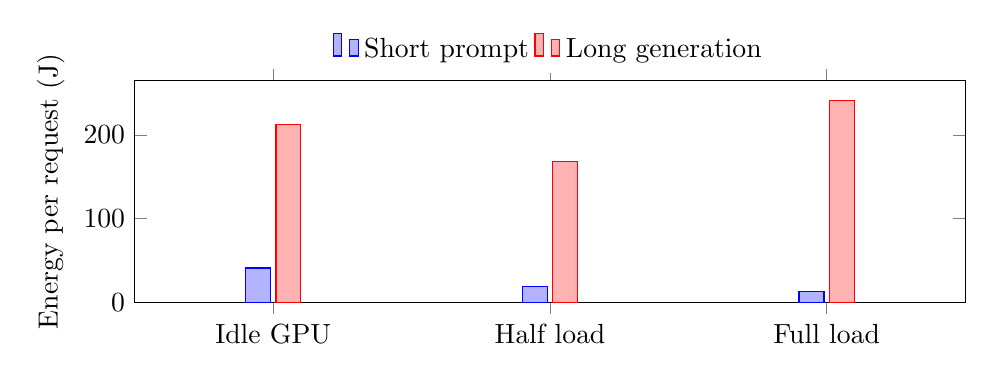
\begin{tikzpicture}
    \begin{axis}[
        ybar, width=\columnwidth, height=4.4cm, ymin=0, bar width=9pt,
        ylabel={Energy per request (J)},
        symbolic x coords={Idle GPU, Half load, Full load}, xtick=data,
        enlarge x limits=0.25,
        legend style={at={(0.5,1.03)}, anchor=south, legend columns=2, draw=none},
      ]
      \addplot coordinates {(Idle GPU, 41) (Half load, 19) (Full load, 13)};
      \addplot coordinates {(Idle GPU, 212) (Half load, 168) (Full load, 241)};
      \legend{Short prompt, Long generation}
    \end{axis}
  \end{tikzpicture}
  \caption{The same two requests under three load levels.}
  \label{fig:load}
\end{figure}

Figure~\ref{fig:load} shows why a per-request figure needs the load around it.
A short prompt gets cheaper as the batch fills, because the fixed cost of each decoding step is shared.
A long generation gets more expensive at full load, because it keeps the batch open while new requests queue behind it.


\section{Related Work}\label{sec:related}

Census studies of inference clusters report where the energy goes at the level of whole services~\cite{kessler2025inference}.
Carbon accounting tools for shared accelerators split energy by time share~\cite{quintero2023carbon}, which is the baseline we compare against.
Work on continuous batching studies throughput and latency~\cite{teller2024batching}.
We add the energy of each request in the batch.

\section{Conclusion}\label{sec:conclusion}

Per-request energy on a shared GPU can be measured to within a few percent, once the power trace is aligned with the kernels that ran.
The load around a request matters as much as the request itself.
\sysname{} and the data set will be released with the camera-ready version.

\bibliographystyle{ACM-Reference-Format}
\bibliography{refs}

\end{document}
